\documentclass[12pt]{article}
\usepackage{fullpage}
\usepackage{amsmath}
\usepackage{hyperref}
\usepackage{graphicx}

\begin{document}
	\begin{center}
		\textbf{\large Superscalar SMIPS} \\
		6.375 Final Project Proposal\\
		30 March 2011 \\
		
		\vspace{\baselineskip}
		
		\emph{Team}: David S. Greenberg and Bhaskar Mookerji
	\end{center}
	
	For our 6.375 final project, we propose to extend an existing superscalar, out-of-order execution processor using Tomasulo's algorithm. There are several approaches we are considering, which could possibly be combined. First, we could augment an existing SMIPS implementation with multiple-instruction dispatch and complex execution units (e.g., floating point and vector modules), exploring various performance tradeoffs. This project will build off of existing implementations for an SMIPS ISA: Nikil Dave's  Bluespec reorder buffer\footnote{\url{http://csg.csail.mit.edu/pubs/memos/Memo-478/memo-478.pdf}.} and other 6.375 explorations in speculative execution in 2005 and 2007\footnote{\begin{itemize}
		\item 2005:~\url{http://csg.csail.mit.edu/6.884/projects/group4-report.pdf}
		\item 2005:~\url{http://csg.csail.mit.edu/6.884/projects/group2-report.pdf}
		\item 2007:~\url{http://csg.csail.mit.edu/6.375/6_375_2007_www/projects/group4_final_report.pdf}
	\end{itemize}}. By starting from an existing project, we will bypass some of the difficulty in verifying and debugging the correctness of an out-of-order execution implementation. Alternatively, we could implement Tomasulo's algorithm using modular refinement, testing each of the primary components (reorder buffer and reserveration stations) in isolation, and extending the tracing framework provided during labs 5 and 6 to help us explore the nondeterministic data flows inherent in the out-of-order design.
	
	Second, we could use high-level abstraction within Bluespec to extend an SMIPS Tomasulo algorithm to a generalized register load-store ISA. The notion here is to preserve the branch instruction and storage processing components of our existing SMIPS architecture, and dynamically generate the execution architecture at Bluespec's compile-time. There is some precedent in this idea within flexible instruction set simulators, which use generic instruction models to target many variations of architectures with complex instruction sets\footnote{For example:~\url{http://portal.acm.org/ft_gateway.cfm?id=1151083&type=pdf}.}. To develop this retargetable ISA processor, we will have to find a reference model that both performs well and is efficient in describing architectures and their instruction sets, and incorporate that abstraction into the instruction fetch stage. The remainder of this project will be an exploration of Bluespec's capabilities in generic decoding and dispatching on differing instruction sets.
	
    \section{High-Level Design}
    
    \begin{figure}[ht]
      \centering
        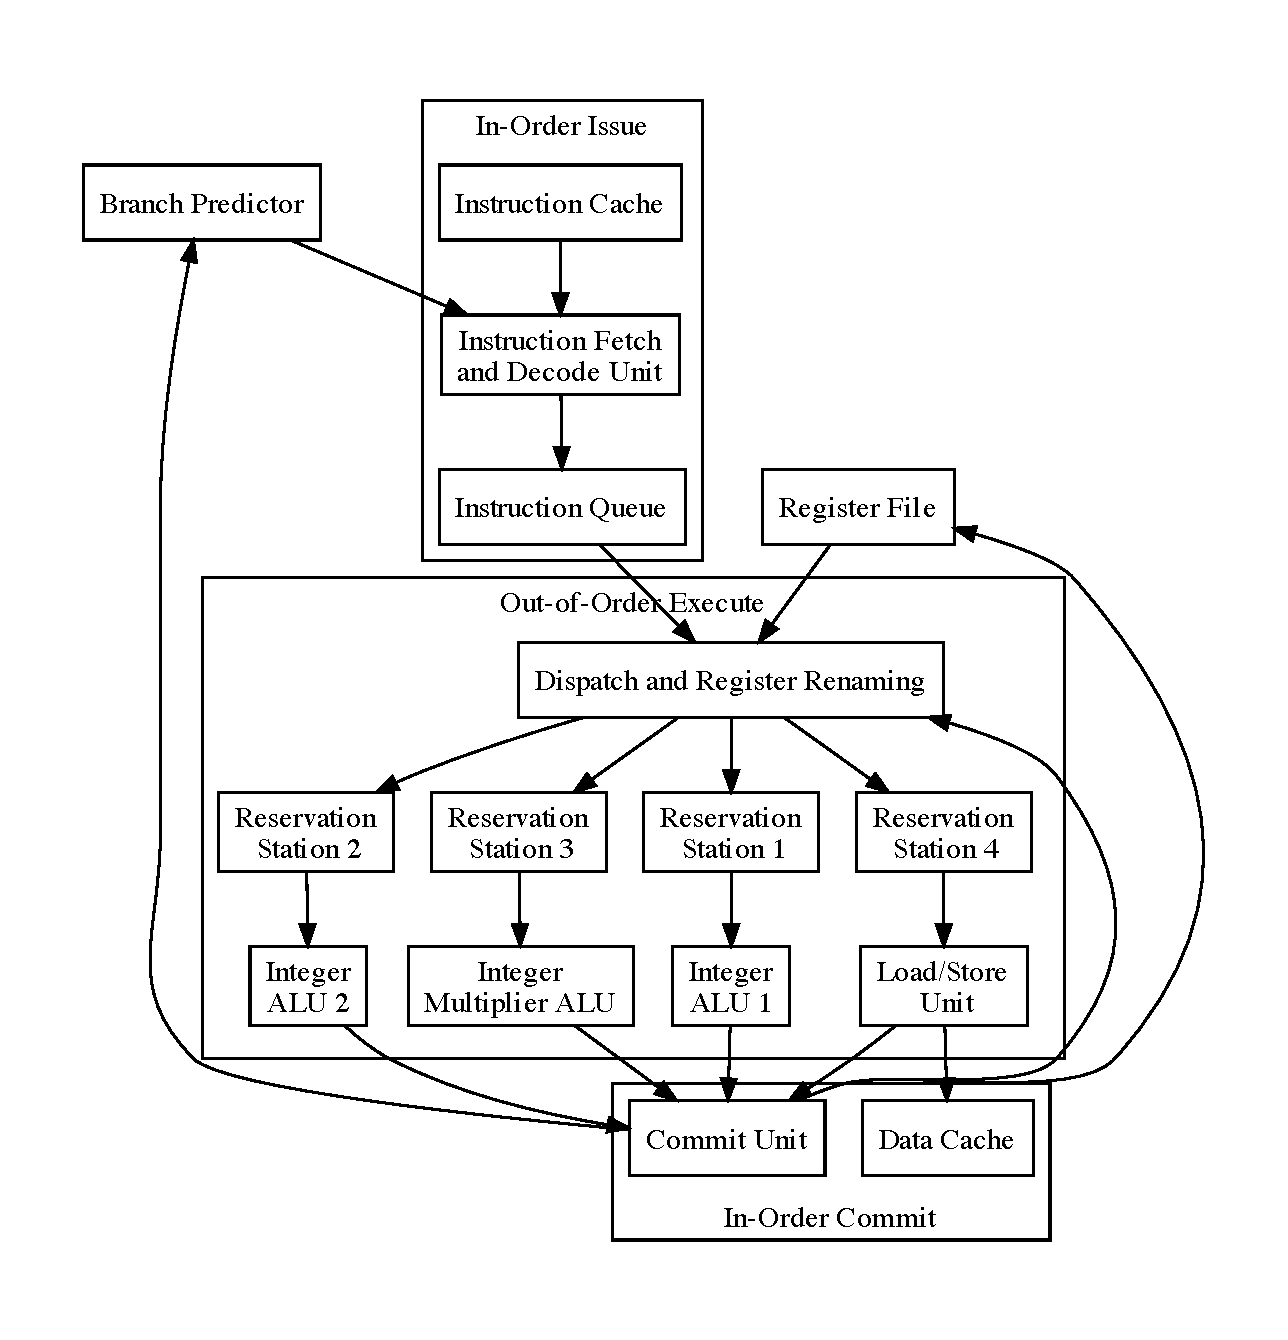
\includegraphics[width=\textwidth]{figures/design.pdf}
        \caption{High-level units.\label{fig:design}}
    \end{figure}
    
    \begin{figure}[ht]
      \centering
        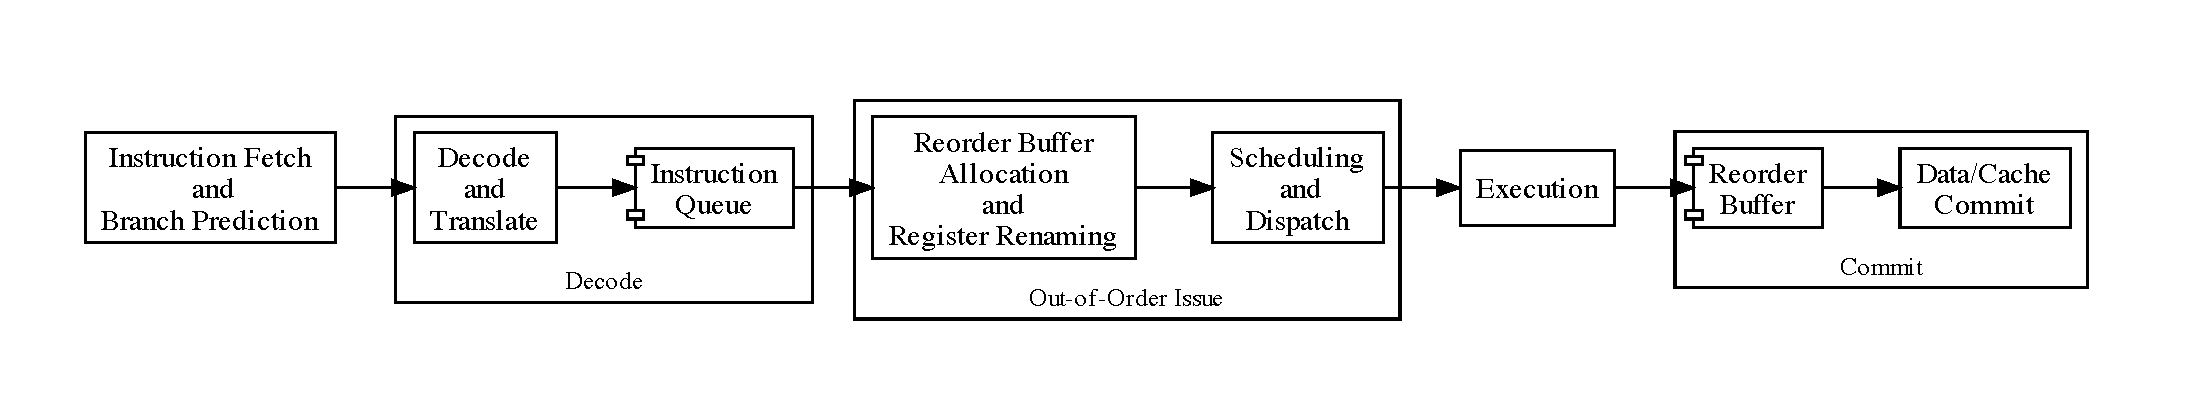
\includegraphics[width=\textwidth]{figures/pipeline.pdf}
        \caption{Pipeline design. \label{fig:pipeline}}
    \end{figure}
    
    Figure~\ref{fig:design} and Figure~\ref{fig:pipeline}
	
\end{document}
